\appendix
\chapter{その他の実験}
\section{夜間TIR画像に対する着色}
TIRカメラは可視光カメラの視界が大きく制限される夜間において優位性を発揮する.したがって,夜間TIR画像の着色は昼間TIR画像の着色よりも実際に利用される可能性が高いシナリオであると考えられる.しかし,同じTIR画像であっても昼間に撮影したTIR画像と夜間に撮影したTIR画像では輝度分布に異なる特徴が表れる.例えば,日照により物体の温度が平均的に高くなる昼間は画像の輝度値が全体的に近い値になるのに対し,気温が下がる夜間は車両のエンジン部等の熱源とその他の部分の輝度差が大きくなる.
本節では夜間TIR画像を各手法を用いて着色し,昼間の可視光画像に変換した際の品質を比較することで,提案手法の夜間TIR画像に対する有効性を検証する.評価に用いるデータセットは夜間TIR画像が含まれるKAIST及びFLIRデータセットとし,テスト画像の枚数はKAISTが15962枚,FLIRが4535枚とする.また,定量評価指標にはFIDを用いる.\par
まず,表\ref{tab:night_image_fid}に定量評価結果を示す.表\ref{tab:night_image_fid}から,提案手法が最も優れたFIDスコアを示しており,昼間可視光画像の分布を再現できていることがわかる.
続いて,図\ref{fig:qualitative_night}に各手法における出力結果を示す.なお,1行目がKAISTデータセット,2行目がFLIRデータセットでの出力結果である.図\ref{fig:qualitative_night}の1行目からは,既存手法では車両が透けているように着色されたり形状に歪みが表れている一方,提案手法では車両が明瞭で自然な色に着色されているほか,人物のシルエットの視認性が向上していることがわかる.また2行目では,画像左側の横行する車両の視認性や中央の車両のテクスチャ品質などから提案手法の優位性が確認でき,全体的に優れた品質の画像を生成できていることがわかる.

\begin{table}[tb]
\centering
\caption{夜間TIR画像を着色した場合の定量評価(FID)}
\label{tab:night_image_fid}
\scalebox{1}{%
\begin{tabular}{l|cc}
\hline
着色手法       & KAIST   & FLIR     \\ \hline
pix2pix      & 168.30  & 90.86    \\
TIC-CGAN     & 108.03  & 74.41    \\
SCGAN        & 142.79  & 80.58    \\
MUGAN        & \underline{93.42}   & \underline{71.88}    \\
提案手法      & \textbf{67.06}   & \textbf{70.15}    \\ \hline
\end{tabular}%
}
\end{table}

\begin{figure}[tb]
    \centering
    \includegraphics[clip, width=1\columnwidth]{images/qualitative_night_jp.pdf}
    \caption{各手法における夜間TIR画像の着色結果}
    \label{fig:qualitative_night}
\end{figure}

\section{ユーザースタディ}
本研究では複数の定量評価手法を用いて提案手法の評価を行なっているが,それらが必ずしも人間から見た画像の品質と一致するとは限らない.そこで,提案手法と既存手法のどちらの着色画像が優れていると感じるかについて主観評価アンケートを実施することで,提案手法の有効性を評価する.被験者は提案手法,既存手法及び参照用のGround-Truthの3枚の画像を一度に提示され,画像中の物体をより正しく把握できると感じた画像を2つの手法の中から選択する.実験にはKAISTデータセットを使用し,比較手法は生成画像の品質が比較的高いMUGAN及びTIC-CGANとする.被験者数は18名で,提案手法とMUGANを比較する25問,提案手法とTIC-CGANを比較する25問の計50問に回答する.
表\ref{tab:user_study}に主観評価アンケートの結果を示す.

\begin{table}[tb]
\centering
\caption{主観評価アンケートの集計結果}
\label{tab:user_study}
\scalebox{1}{
\begin{tabular}{cc|cc|cc}
\hline
\multirow{2}{*}{比較手法} & \multirow{2}{*}{回答数} & \multicolumn{2}{c|}{テスト画像全体} & \multicolumn{2}{c}{有意差がある画像} \\
                          &                  & 枚数[枚]   & 割合[\%]  & 枚数[枚] & 割合[\%] \\ \hline
\multirow{3}{*}{TIC-CGAN} & 「提案手法が良い」が多い     & 25        & 100      & 23       & 100    \\
                          & 「TIC-CGANが良い」が多い    & 0         & 0        & 0        & 0      \\ 
                          & 回答数が等しい     & 0         & 0        & -        & -        \\  \hline
\multirow{3}{*}{MUGAN}    & 「提案手法が良い」が多い     & 18        & 72     & 9        & 90   \\
                          & 「MUGANが良い」が多い       & 5         & 20     & 1        & 10    \\ 
                          & 回答数が等しい     & 2         & 8      & -        & -        \\ \hline
\end{tabular}%
}
\end{table}

表\ref{tab:user_study}中央は,全てのテスト画像に関する集計結果である.ここからTIC-CGAN,MUGANともに「提案手法が良い」と回答した割合が「既存手法が良い」と回答した割合を上回っていることがわかる.
また,被験者が「提案手法が良い」または「既存手法が良い」と回答する割合がそれぞれ1/2であるという帰無仮説と,それぞれの割合は異なるという対立仮説を立て,帰無仮説が有意水準5\%で棄却されるか否かによって回答に有意差があるかを判定し,回答に有意差があった画像について集計した結果が表\ref{tab:user_study}右側である.これより,有意差がある画像についても「提案手法が良い」と回答した割合の方が大きいことがわかる.\par

続いて,図\ref{fig:existing_better}に主観評価アンケートで「既存手法が良い」と回答した割合が高かった画像の例を,図\ref{fig:proposed_better}に「提案手法が良い」と回答した割合が高かった画像の例を示す.

\begin{figure}[tb]
    \centering
    \caption{「既存手法が良い」と回答した割合が高かった画像}
    \label{fig:existing_better}
    \subfigure[TIR]{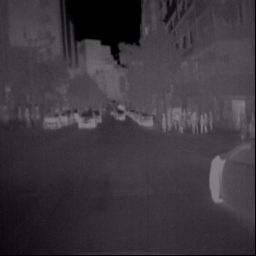
\includegraphics[clip, width=0.24\columnwidth]{images/user_study/existing_better/img24_TIR.png}}
    \subfigure[Ground-Truth]{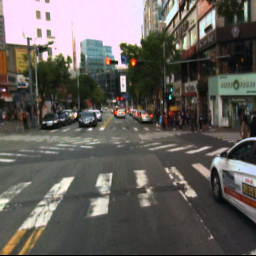
\includegraphics[clip, width=0.24\columnwidth]{images/user_study/existing_better/img24_gt.jpg}}
    \subfigure[提案手法]{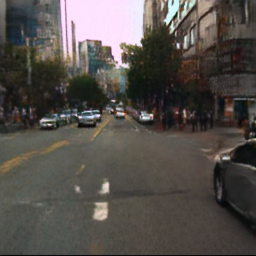
\includegraphics[clip, width=0.24\columnwidth]{images/user_study/existing_better/img24_proposed.jpg}}
    \subfigure[既存手法(MUGAN)]{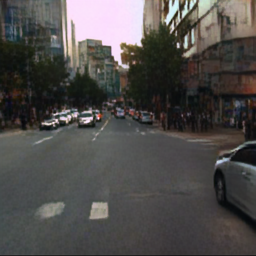
\includegraphics[clip, width=0.24\columnwidth]{images/user_study/existing_better/img24_mu.jpg}}
\end{figure}

\begin{figure}[tb]
    \centering
    \caption{「提案手法が良い」と回答した割合が高かった画像}
    \label{fig:proposed_better}
    \subfigure[TIR]{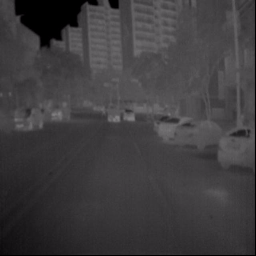
\includegraphics[clip, width=0.24\columnwidth]{images/user_study/proposed_better/img14_TIR.png}}
    \subfigure[Ground-Truth]{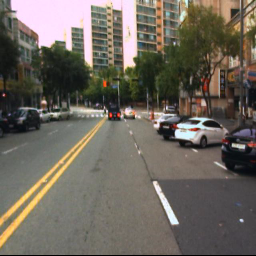
\includegraphics[clip, width=0.24\columnwidth]{images/user_study/proposed_better/img14_gt.jpg}}
    \subfigure[提案手法]{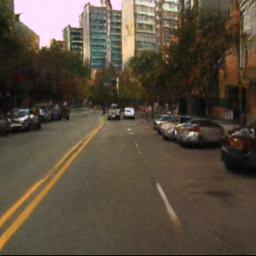
\includegraphics[clip, width=0.24\columnwidth]{images/user_study/proposed_better/img14_proposed.jpg}}
    \subfigure[既存手法(MUGAN)]{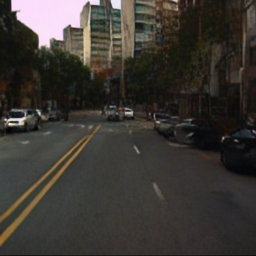
\includegraphics[clip, width=0.24\columnwidth]{images/user_study/proposed_better/img14_mu.jpg}}
\end{figure}

「既存手法が良い」との回答が多かった画像には,図\ref{fig:existing_better}のように物体の視認性は同程度であるが,提案手法の方が既存手法よりもテクスチャに歪みが見られるものが多く見られた.
一方で「提案手法が良い」との回答が多かった画像は図\ref{fig:proposed_better}のように,既存手法よりも提案手法の方が車両などの前景物体の輪郭がはっきりと確認できるものが多い傾向にあった.以上を踏まえると,提案手法は既存手法において前景物体の視認性が低くなってしまうような入力に対して特に有効であると考えられる.

\section{学習データとテストデータの組み合わせの変更}
本節では学習データが与える出力画像への影響を調査するため,学習データとテストデータの組み合わせを変更して着色画像の生成を行う.学習に用いたデータセットのテスト画像に加え,学習に用いなかったデータセットのテスト画像をモデルに入力すること.\par
図\ref{fig:dataset_swap}にデータセットの組み合わせを変更した際の着色画像の変化を示す.

\begin{figure}[tb]
    \centering
    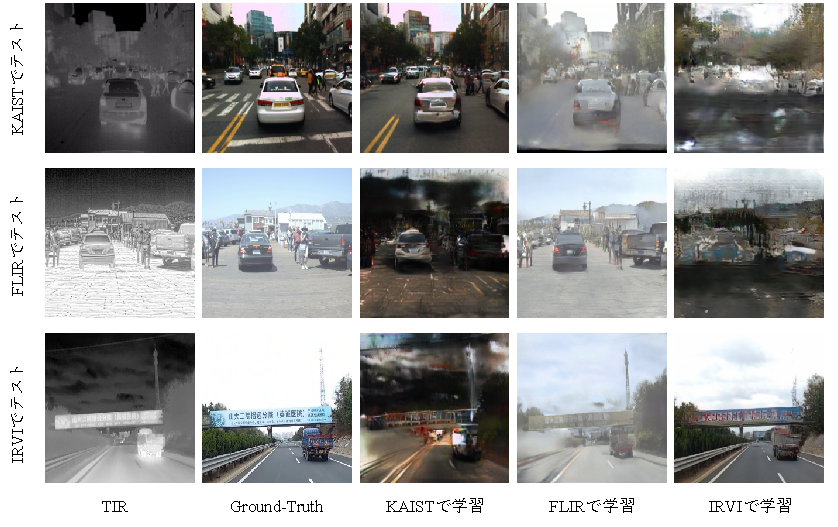
\includegraphics[clip, width=1\columnwidth]{images/dataset_swap.pdf}
    \caption{学習データセットとテストデータセットの組み合わせを変更した際の着色画像の変化}
    \label{fig:dataset_swap}
\end{figure}

図\ref{fig:dataset_swap}から,学習データセットとテストデータセットが異なると生成画像の品質が著しく悪化することがわかる.考えられる品質悪化の原因の一つとして,データセット間の輝度分布の違いが挙げられる.
例えば,FLIRやIRVIは全体的に高コントラストであるため空の領域に比較的輝度が高い領域が存在する一方で,KAISTは全体的に低輝度・低コントラストであるため空の領域の輝度はほとんど0になっている.そのため,KAISTで学習したモデルに他のデータセットの画像を入力すると輝度差によりモデルが混乱し,空の領域を黒く塗りつぶすような不適切な着色が行われたと考えられる.\par
また,他の原因としてはデータセットに含まれるシーンのバリエーションの違いが挙げられる.
図\ref{fig:dataset_swap}では特にIRVIデータセットで学習したモデルの出力画像に大きな歪みが認められるが,KAISTやFLIRが比較的多様なシーンを含むデータセットであるのに対してIRVIが単一のシーンのみを含むデータセットであり,汎化性能が低くなったためだと考えられる.